% 04-rezultati.tex — Results (TASK §F.5). Every number: data/raw/lab_session_01092026_020000/telemetry/*.json.
\section{Rezultati i analiza}
\label{sec:rezultati}

\subsection{Što se uspoređuje s čim}

Zapis kutova sadrži pet stupaca po zglobu, pa usporedba bilo koja dva daje broj
koji izgleda kao vjernost praćenja. Naredba naspram stvarnog kuta robota mjeri
samo koliko dobro servo slijedi vlastitu zadanu vrijednost, ravnodušno na to
kreće li se čovjek uopće; sirovi ulazni kanal naspram naredbe mjeri pojačanje iz
jednadžbe~(\ref{eq:mapiranje}). Vjernost oponašanja zato definiramo kao odnos
\emph{kuta ruke izraženog u stupnjevima zgloba robota} --- dakle nakon pojačanja
i inverzije --- i kuta koji je robot doista dosegnuo. Uz nju izvještavamo i
pogrešku nakon uklanjanja procijenjenog faznog pomaka, jer sustav koji savršeno
prati, ali kasni, inače biva kažnjen kao netočan.

\subsection{Uzorkovanje i latencija obrade}

Okvir predstavlja jedno mjerenje poza svih triju krutih tijela u istom trenutku. Optički
ih sustav isporučuje na 120 Hz, a razmak između uzastopnih okvira iznosi
8,37 $\pm$ 2,96 ms (slika~\ref{fig:kvaliteta}, gore), dakle uzorkovanje je stabilno
oko nazivne vrijednosti od 8,33 ms. Latencija obrade --- vrijeme od isporuke
okvira upravljačkom računalu do slanja naredbe robotu --- iznosi 3,0--4,0 ms u
medijanu, uz p99 između 8,7 i 10,5 ms u pokusima praćenja
(slika~\ref{fig:kvaliteta}, dolje; tablica~\ref{tab:pregled}). Jedini je izlet pokus s
programskim zaustavljanjem, gdje p99 doseže 14,8 ms. Podrhtavanje kašnjenja
(\emph{jitter}), mjereno kao standardna devijacija latencije, ostaje između 2,3
i 3,5 ms. Uz raspoloživih 8 ms po taktu medijan troši manje od polovine tog budžeta,
dok ga u najviše 1\,\% taktova obrada premašuje. Izmjereni takt petlje od 123,9 do 124,7 Hz, tik
ispod nazivnih 125 Hz, pokazuje da su ta prekoračenja apsorbirana bez ispada, pa robot nijednom
nije ostao bez naredbe.

\begin{figure}[htbp]
  \centering
  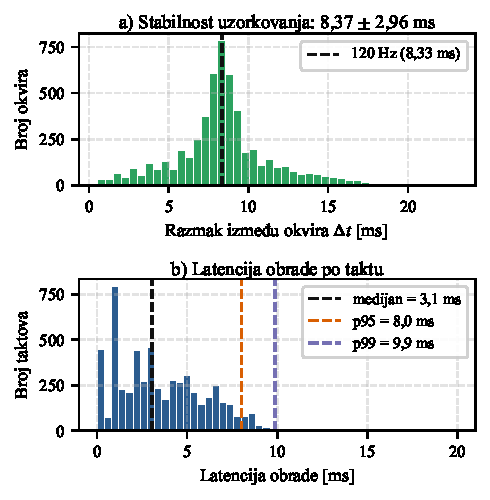
\includegraphics[width=\columnwidth]{figures/signal_quality.pdf}
  \caption{Kvaliteta ulaznog signala i brzina obrade (T1a). Gore je prikazan razmak između
  uzastopnih okvira sustava OptiTrack, a dolje latencija obrade po taktu s
  medijanom, 95. i 99. percentilom.}
  \label{fig:kvaliteta}
\end{figure}

\begin{table}[H]
  \caption{Pregled karakterističnih pokusa. Latencija je vrijeme obrade jednog
  okvira unutar računala i ne uključuje optički put ni mrežu do njega;
  $f_\text{ul}$ je efektivna frekvencija osvježavanja kanala ruke na
  upravljačkoj petlji od 125 Hz.}
  \label{tab:pregled}
  \centering\small
  \begin{tabular}{l rrrrr}
\hline
\textbf{Pokus} & \small $t$ & \small $f_\text{ul}$ & \small med. & \small p95 & \small p99 \\
 & \small [s] & \small [Hz] & \small [ms] & \small [ms] & \small [ms] \\
\hline
T1a --- prirodni tempo & 45 & 57 & 3,1 & 8,0 & 9,9 \\
T1b --- prolaz po zglobovima & 45 & 47 & 3,1 & 7,6 & 8,7 \\
T2a --- filtar One-Euro & 30 & 49 & 3,1 & 7,7 & 9,1 \\
T6 --- nagli pokreti & 30 & 53 & 3,1 & 8,2 & 10,5 \\
\hline
\end{tabular}

\end{table}

Drugi stupac tablice nosi nalaz koji se prenosi kroz cijelo poglavlje. Kanali
ruke stizali su na upravljačku petlju efektivno 31--73 Hz, ovisno o pokusu, a ne
na punih 120 Hz koliko emitira sustav Motive. Uzrok je u strukturi toka, a ne u
gubitku. Datagrami stižu na oko 500 Hz, dakle otprilike četiri po okviru, a dvije
trećine ih dolazi izvan redoslijeda (u pokusu T1a 11\,338 od 17\,011). Uz politiku
najnovijeg okvira svaki pojedini kanal ruke time se osvježava rjeđe od izvorišnog
takta. Na preostalim taktovima petlja nije imala novu vrijednost i zadržavala je
prethodnu naredbu. Posljedica je
mjerljiva jer su filtri projektirani za 125 Hz radili na upola rjeđem ulazu, pa
zaglađuju jače nego što im parametri nalažu.

\subsection{Vjernost oponašanja}

Slika~\ref{fig:pracenje} prikazuje dvadeset sekundi pokusa T1a po svih šest
zglobova. Robot prati oblik pokreta na svakom zglobu; vidljivi su blago
zaglađivanje amplitude i sustavni fazni pomak.

\begin{figure*}[t]
  \centering
  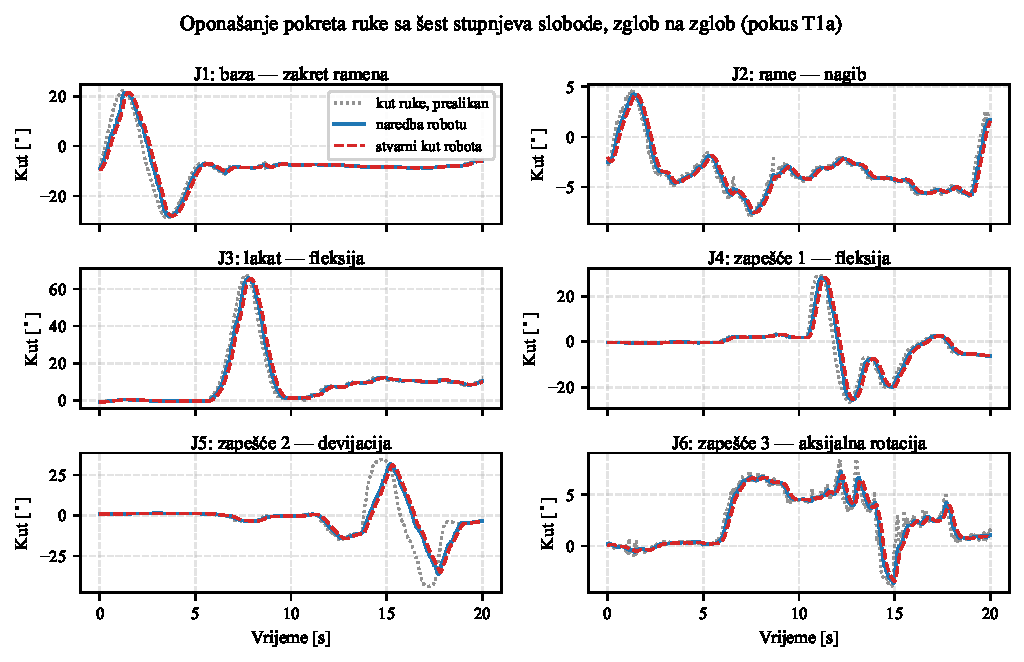
\includegraphics[width=\textwidth]{figures/tracking_6dof_time.pdf}
  \caption{Oponašanje u stvarnom vremenu sa šest stupnjeva slobode (pokus T1a) s
  prikazom kuta ruke preslikanog u stupnjeve zgloba, poslane naredbe i stvarnog kuta robota.}
  \label{fig:pracenje}
\end{figure*}

Brojčano to daje tablica~\ref{tab:vjernost}. Pri prirodnom tempu pogreška nakon
uklanjanja faznog pomaka iznosi 0,36--3,00$^\circ$ po zglobu, uz korelaciju
0,68--0,95. Najveće pogreške ima lakat, i to ne slučajno jer ima najveći raspon
pokreta i pojačanje 1,5, pa se ista relativna pogreška preslikava u veći
apsolutni iznos. Najmanju ima aksijalna rotacija zapešća, čiji je raspon i
najuži.

\begin{table*}[t]
  \caption{Vjernost oponašanja po zglobu usporedbom kuta ruke i stvarnog kuta robota.
  RMSE$_\text{p}$ je pogreška nakon uklanjanja faznog pomaka $\tau$.}
  \label{tab:vjernost}
  \centering\small
  \begin{tabular}{l rrrr rrrr}
\hline
\textbf{Zglob} & \multicolumn{4}{c}{\textbf{T1a --- prirodni tempo}} & \multicolumn{4}{c}{\textbf{T1b --- prolaz po zglobovima}} \\
 & \small RMSE & \small RMSE$_\text{p}$ & \small $\tau$ & \small $r$ & \small RMSE & \small RMSE$_\text{p}$ & \small $\tau$ & \small $r$ \\
 & \small [$^\circ$] & \small [$^\circ$] & \small [ms] &  & \small [$^\circ$] & \small [$^\circ$] & \small [ms] & \\
\hline
J1 (\textit{base}, rotacija ramena) & 3,50 & 0,84 & 305 & 0,900 & 6,00 & 2,63 & 530 & 0,939 \\
J2 (\textit{shoulder}, elevacija ramena) & 1,92 & 0,39 & 257 & 0,940 & 2,43 & 0,49 & 265 & 0,973 \\
J3 (\textit{elbow}, lakat) & 8,66 & 3,00 & 385 & 0,850 & 11,46 & 4,92 & 554 & 0,824 \\
J4 (\textit{wrist 1}, fleksija zapešća) & 4,44 & 1,57 & 337 & 0,806 & 4,23 & 1,33 & 337 & 0,903 \\
J5 (\textit{wrist 2}, devijacija zapešća) & 6,89 & 2,97 & 602 & 0,683 & 10,69 & 6,24 & 787 & 0,683 \\
J6 (\textit{wrist 3}, aksijalna rotacija) & 1,00 & 0,36 & 241 & 0,952 & 1,36 & 0,53 & 241 & 0,954 \\
\hline
\multicolumn{9}{l}{\small Efektivna frekvencija ulaza: 57 Hz (T1a), 47 Hz (T1b); upravljačka petlja 125 Hz.} \\
\end{tabular}

\end{table*}

U pokusu prolaza po zglobovima (T1b), gdje operater izvodi izolirano gibanje svakog pojedinog zgloba kroz puni raspon, pogreška iznosi 0,49--6,24$^\circ$, a fazni pomak 241--787 ms. Veće vrijednosti pogreške na laktu (J3) i rotaciji ramena (J1) proizlaze iz znatno većih pojedinačnih amplituda pri izoliranom pokretu. Efektivna frekvencija ulaza u T1b iznosila je 47 Hz, jer se između pokreta pojedinih segmenata ruka kratko zadržava u referentnom položaju.

Jedan izuzetak traži objašnjenje. Devijacija zapešća (J5) ima najlošiju
korelaciju u oba pokusa, 0,683, iako joj pogreška nije najveća. Uzrok je
kinematičke naravi jer devijacija zapešća čovjeka i zglob \emph{wrist 2} robota nemaju
zajedničko središte rotacije, pa se isti pokret ruke na robotu ostvaruje
kombinacijom koja djelomično curi u susjedne kanale. Operater je istu pojavu
opisao neovisno o mjerenju --- rotacije u ramenu i laktu doživio je kao znatno
prirodnije od zapešća. Ostala četiri zgloba imaju korelaciju iznad 0,90 u oba
pokusa.

Stabilnost je bila jednolika kroz cijelu sesiju. Kroz 21 uzastopni pokus,
ukupno nešto više od deset minuta gibanja, upravljačka petlja nije izgubila
takt, veza RTDE nije pala, a referentna poza robota između pokusa nije se
pomaknula, pa kumulativnog odstupanja nema.

\subsection{Odakle dolazi kašnjenje}

Ukupni fazni pomak ruka--robot na laktu iznosi 385 ms. Pojedini su stupnjevi procijenjeni kao razlike zaostajanja između uzastopnih parova signala u lancu, od ulaznog kuta preko filtrirane vrijednosti i poslane naredbe do kuta očitanog s enkodera (tablica~\ref{tab:budzet}).

\begin{table}[H]
  \caption{Razlaganje ukupnog kašnjenja na laktu (pokus T1a) na doprinose filtra, sigurnosnog sloja i pogona. Zaostajanje $\tau$ aditivno je po lancu, dok stupac RMSE prikazuje prirast pogreške po stupnju, a ne aditivni udio.}
  \label{tab:budzet}
  \centering\small
  \begin{tabular}{l rr}
\hline
\textbf{Stupanj / uzrok (J3)} & \small $\tau$ [ms] & \small RMSE [$^\circ$] \\
\hline
Filtar (\textit{One-Euro}) & 200 & 4,22 \\
Sigurnosni sloj (brzina) & 73 & 2,04 \\
Pogon robota (\textit{lookahead}) & 112 & 2,40 \\
\hline
\textbf{Ukupno (ruka $\rightarrow$ robot)} & \textbf{385} & \textbf{8,66} \\
\hline
\end{tabular}

\end{table}

Regulacija pogona robota doprinosi 112 ms, što odgovara postavljenom parametru predviđanja (\emph{lookahead}) od 100 ms u pozivu \texttt{servoj} uvećanom za elektromehanički odziv motora. Taj stupanj ostaje konstantan kroz cijelu sesiju, između 112,3 i 112,5 ms u 19 od 21 pokusa, neovisno o filtru, sigurnosnim granicama i dodanom kašnjenju. Sigurnosni sloj ograničenja brzine dodaje daljnjih 73 ms uslijed zasićenja na naglim dijelovima zamaha ruke. Preostalih 200 ms otpada na fazno kašnjenje filtra One-Euro pri potiskivanju šuma, dakle nešto više od polovine ukupnog odziva, a zajedno sa sigurnosnim slojem oko sedamdeset posto. Kroz sve pokuse s tim filtrom njegov udio ostaje u rasponu 48 do 59\,\%. Filtriranje signala time određuje odziv više nego mrežni prijenos ili računalna obrada, čime se potvrđuje teorijsko upozorenje da niskopropusno filtriranje unosi fazno kašnjenje \cite[str.~2]{zhu2022}, dok lokalna mreža i programski kod s latencijom od 3 ms ne predstavljaju usko grlo.

\subsection{Usporedba filtara na stvarnom robotu}

Četiri su filtra izmjerena na robotu istim pokretom (slika~\ref{fig:filtri},
tablica~\ref{tab:filtri}). Rezultat je podijeljen. Objektivno, najmanju pogrešku
i najkraće kašnjenje daje rad bez filtra (1,00$^\circ$, 217 ms), a najgori je
Butterworth (2,79$^\circ$, 682 ms). Subjektivno, operater je bez oklijevanja
rangirao One-Euro kao najbolji, a Butterworth kao najgori, dok je rad bez filtra
opisao kao nervozan i skokovit.

\begin{figure*}[t]
  \centering
  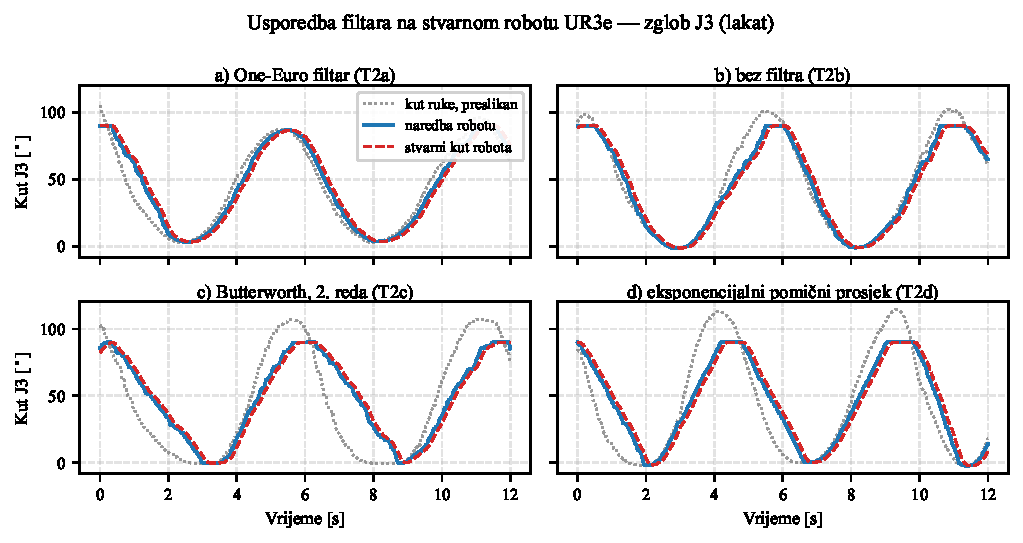
\includegraphics[width=0.95\textwidth]{figures/filter_real_robot.pdf}
  \caption{Sirovi i filtrirani signal na stvarnom robotu za zglob J3
  (T2a--T2d) s prikazom kuta ruke, naredbe nakon filtra i kuta koji je robot dosegnuo.}
  \label{fig:filtri}
\end{figure*}

\begin{table}[H]
  \caption{Filtri na stvarnom robotu (T2a--T2d) uz parametre One-Euro
  $f_{c,\min}=1{,}0$ Hz i $\beta=0{,}007$; Butterworth 2.~reda $f_c=6$ Hz;
  eksponencijalni pomični prosjek $\alpha=0{,}2$.
  $\overline{\text{RMSE}}_\text{p}$ je srednja pogreška po šest zglobova nakon
  uklanjanja faznog pomaka, a stupac ograničenja brzine broj taktova u kojima je
  sloj djelovao. Rang je kvalitativna ocjena dvaju sudionika i stoji uz objektivne
  stupce kao njihova dopuna, ne kao mjerena veličina.}
  \label{tab:filtri}
  \centering\small
  \begin{tabular}{l rrr c}
\hline
\textbf{Filtar} & \small $\overline{\text{RMSE}}_\text{p}$ & \small $\tau_\text{J3}$ & \small Ogr. brz. & \textbf{Rang} \\
 & \small [$^\circ$] & \small [ms] & \small [takt] & \\
\hline
One-Euro & 1,19 & 353 & 621 & 1. \\
Bez filtra & 1,00 & 217 & 1003 & 3. \\
Butterworth & 2,79 & 682 & 932 & 4. \\
EMA & 2,40 & 282 & 1235 & 2. \\
\hline
\end{tabular}

\end{table}

Ta razlika nije proturječje nego mjerenje dviju različitih stvari. Bez filtra
sustav prenosi i mikrootklone, pa sloj ograničenja brzine okida na 1003 takta
umjesto na 621 s filtrom One-Euro; robot se zbog toga trza, iako je u prosjeku
bliže ruci. Butterworth pokazuje najlošije oboje jer njegova fiksna granična
frekvencija, na upola rjeđem ulazu od projektiranog, prigušuje i koristan
sadržaj. Izvanmrežna usporedba na ranijim snimkama pokazuje jednaku strukturu.
One-Euro uklanja do 56,6\,\% podrhtavanja kuta uz 50--100 ms kašnjenja, dok
Butterworth i eksponencijalni pomični prosjek daju 25--42 ms kašnjenja uz
slabije prigušenje.

\subsection{Sigurnosni slojevi}

Svaki je sigurnosni sloj ispitan zasebno uz eksperimentalne granice odabrane tako da sigurno okinu unutar radnog raspona (tablica~\ref{tab:sigurnost}, slika~\ref{fig:sigurnost}). Ograničenje brzine (T3a) djelovalo je na 23,8\,\% taktova (745 taktova) i naredbu je zasitilo glatko, bez oscilacija. Ograničenje raspona (T3b) zadržalo je zglob točno na granici kroz 13,0\,\% taktova (406 taktova) i oslobodilo ga čim se ruka vratila u dopušteni prostor. Zaustavljanje u nuždi (T3d) ispitano je programskim okidanjem u desetoj sekundi uz pritisak sigurnosne sklopke na upravljačkoj jedinici robota, čime su zglobovi zamrznuti na točno 50,1\,\% taktova (1252 takta).

\begin{table}[H]
  \caption{Sigurnosni slojevi sa zadanim granicama i udjelima taktova u kojima je pojedini sloj djelovao.}
  \label{tab:sigurnost}
  \centering\small
  \begin{tabular}{l l l rr}
\hline
\textbf{Pokus} & \textbf{Sloj} & \textbf{Granica} & \small Takt & \small [\%] \\
\hline
T3a & Ogr. brzine & $25^\circ/\text{s}$ & 745 & 23,8 \\
T3b & Ogr. raspona & $\pm 25^\circ$ & 406 & 13,0 \\
T3c & Okluzija & okluzija markera & 617 & 16,5 \\
T3d & Zaustavljanje & $t=10$ s & 1252 & 50,1 \\
T6 & Nagli pokret & $150^\circ/\text{s}$ & 174 & 4,6 \\
\hline
\end{tabular}

\end{table}

\begin{figure*}[t]
  \centering
  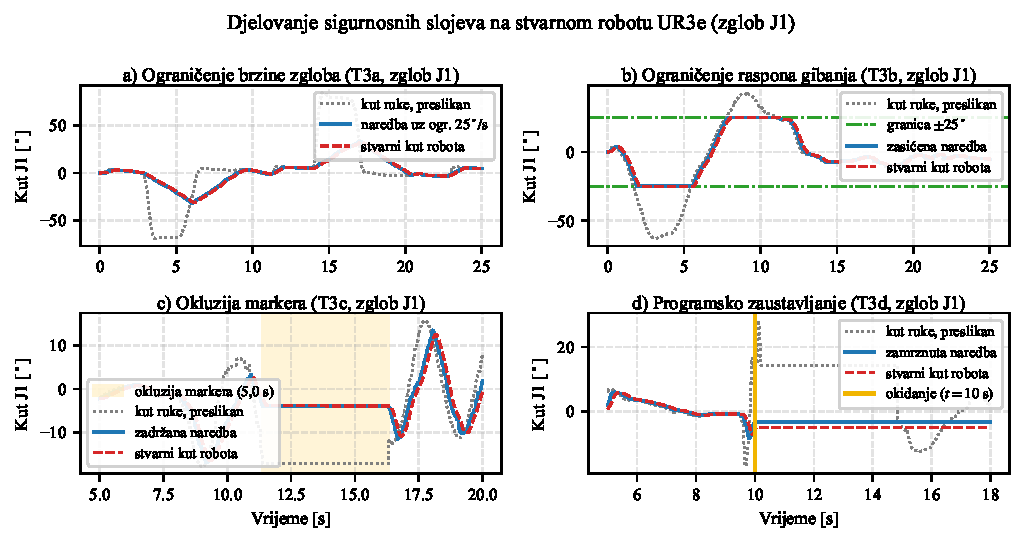
\includegraphics[width=0.95\textwidth]{figures/safety_events.pdf}
  \caption{Djelovanje sigurnosnih slojeva kroz vrijeme na zglobu baze J1 za a) ograničenje brzine zgloba na $25^\circ/\text{s}$ (T3a), b) ograničenje raspona gibanja na $\pm 25^\circ$ (T3b), c) zadržavanje stanja pri okluziji markera (T3c) te d) zaustavljanje u nuždi u $t=10\text{ s}$ (T3d).}
  \label{fig:sigurnost}
\end{figure*}

Okluzija markera (T3c) pokazala je specifičnost višesegmentnog praćenja krutih tijela. Pri namjernom zaklanjanju markera nadlaktice u trajanju od 5,0 s (od 11,37 do 16,32 s pokusa, ukupno 617 uzastopnih taktova, odnosno 16,5\,\% trajanja), kinematički most zadržao je posljednju važeću pozu nadlaktice. Zglobovi ramena i lakta (J1, J2, J3) ostali su zamrznuti na konstantnim kutovima, dok su zglobovi zapešća (J4, J5, J6) nesmetano nastavili pratiti kretanje šake jer njezini markeri nisu bili zaklonjeni. Time se sprječava nagli prekid cjelokupnog rada pri lokalnom gubitku vidljivosti pojedinog segmenta.

\subsection{Nagle promjene i dodano kašnjenje}

Kako bi se teorijski i analitički izoliralo dinamičko ponašanje filtersko-sigurnosnog lanca na kanonske poremećaje, provedena je simulacija odziva na idealnu skokovitu pobudu od 40$^\circ$ i kratki impuls (slika~\ref{fig:dinamika}b). Filtar prati skok unutar nekoliko desetaka milisekundi, a sigurnosni sloj ga pretvara u rampu određenu dopuštenom brzinom zgloba; kratki impuls sloj propušta samo djelomično, čime se sprječava da se vršna brzina ruke prenese na pogone robota.

Analitički nalaz izravno je potvrđen fizikalnim pokusom na robotu UR3e u pokusu T6, gdje je operater izveo pet uzastopnih naglih trzaja ruke (videozapis \texttt{T6\_step\_response.mp4}). Sustav je brze pokrete pratio stabilno, bez pojave oscilacija i bez premašivanja. Sloj ograničenja brzine pritom je djelovao na 178 taktova (4,6\,\%), dok je pogreška nakon uklanjanja faznog pomaka iznosila 1,23$^\circ$ uz fazni pomak od 257 ms. Usporedba simulacijskog i eksperimentalnog odziva dokazuje da robot ne pokušava reproducirati nekontroliranu vršnu brzinu ruke, nego joj se glatko približava po fizikalno sigurnoj putanji.

\begin{figure*}[t]
  \centering
  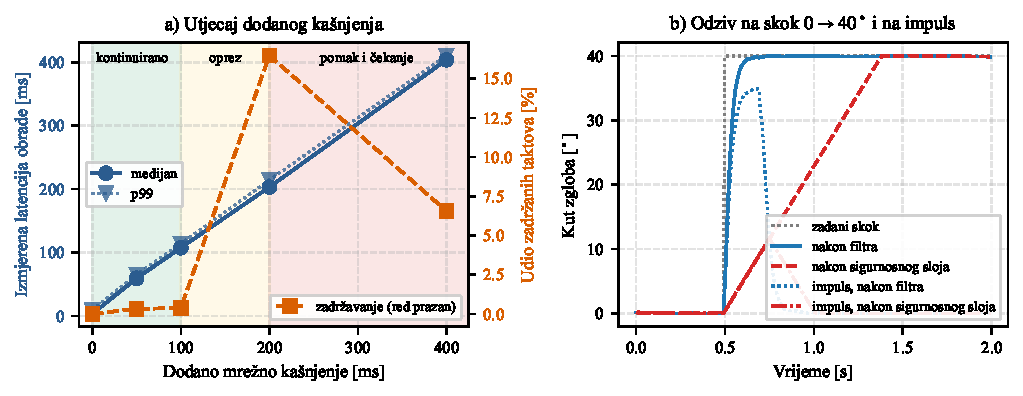
\includegraphics[width=0.95\textwidth]{figures/dynamics.pdf}
  \caption{Dinamičko ponašanje lanca. Lijevo je prikazana izmjerena latencija i udio taktova sa zadržanim izlazom pri umjetno dodanom kašnjenju (T4a--T4e) uz pojaseve načina vođenja iz poglavlja~\ref{sec:rasprava}, a desno simulacijski odziv filtra i sigurnosnog sloja na skok i impuls, komplementaran eksperimentalnom pokusu T6 na robotu.}
  \label{fig:dinamika}
\end{figure*}

Umjetno kašnjenje ubačeno je između prijema i obrade u pet nominalnih iznosa od 0 do
400 ms (slika~\ref{fig:dinamika}a, tablica~\ref{tab:kasnjenje}). Izmjerena
latencija obrade strogo monotono prati zadanu vrijednost (3,1, 59,3, 107,4, 203,2 i
403,9 ms u medijanu) uz raspon od p95 do p99 uži od 7 ms u svakoj točki.
Budući da se umjetno kašnjenje unosi u međuspremnik prije izračuna kutova, ono
se izravno pribraja baznom dinamičkom odzivu sustava od 385 ms. Tako ukupno
fizikalno kašnjenje od pokreta ruke do odziva robota ($\tau_\text{ukupno}$)
monotono raste od 385 ms pri baznom radu do čak 785 ms pri dodanih 400 ms,
što iznosi gotovo cijelu sekundu zaostajanja.

Pritom desna os na slici~\ref{fig:dinamika}a i zadnji stupac tablice~\ref{tab:kasnjenje}
prikazuju udio taktova sa zadržanim izlazom uslijed privremenog pražnjenja međuspremnika.
Za razliku od latencije koja strogo monotono raste, zadržavanje dostiže vrhunac
pri 200 ms dodanog kašnjenja (618 taktova, odnosno 16,5\,\%), dok pri 400 ms pada na
246 taktova (6,6\,\%). Ovaj prividni paradoks posljedica je elastičnosti reda čekanja:
pri 200 ms red sadrži oko 25 okvira pa je osjetljiviji na mrežni jitter dolaznih UDP paketa,
što povremeno uzrokuje kratkotrajno pražnjenje reda u pojedinačnom taktu petlje na 125 Hz.
Pri 400 ms red je dvostruko dublji (oko 50 okvira) i uspješnije amortizira mrežna
kolebanja, pa je broj taktova bez novog okvira znatno manji unatoč većem ukupnom kašnjenju.

\begin{table}[H]
  \caption{Niz mjerenja s dodanim kašnjenjem (T4a--T4e). Stupac $\tau_\text{ukupno}$
  prikazuje ukupno kašnjenje ruka--robot kao zbroj baznog dinamičkog odziva
  (385 ms) i dodanog kašnjenja. Prag starosti signala podiže se uz dodano
  kašnjenje jer starost uključuje i to kašnjenje, pa bi fiksnih 150 ms trajno
  držalo fail-safe i onemogućilo mjerenje.}
  \label{tab:kasnjenje}
  \centering\small
  \begin{tabular}{rrrrrr}
\hline
\small Dodano & \small Medijan & \small p95 & \small $\tau_\text{ukupno}$ & \small Prag & \small Zadrž. \\
\small [ms] & \small [ms] & \small [ms] & \small [ms] & \small [ms] & \small [takt] \\
\hline
0 & 3,1 & 7,6 & 385 & 150 & 0 \\
50 & 59,3 & 63,9 & 435 & 300 & 12 \\
100 & 107,4 & 112,0 & 485 & 400 & 14 \\
200 & 203,2 & 209,6 & 585 & 600 & 618 \\
400 & 403,9 & 408,7 & 785 & 900 & 246 \\
\hline
\end{tabular}

\end{table}

\subsection{Otpornost na gubitak paketa}

Pokusi T5a--T5e izvedeni su na stvarnom robotu (videozapisi \texttt{T5a\_packet\_loss\_0pct.mp4} do \texttt{T5e\_packet\_loss\_30pct.mp4}). Gubitak paketa modeliran je deterministički nad baznom putanjom pokusa T5a, tako da svih pet stopa od 0 do 30\,\% dijeli identične polazne uvjete. Takav postupak izolira čist utjecaj mrežnog gubitka od prirodne varijance ljudskog pokreta među pojedinačnim izvođenjima (tablica~\ref{tab:gubitak}).

Pokazatelji potvrđuju visoku robusnost jer starost signala u 95. percentilu monotono raste s 7,5 na 19,7 ms, dok pogreška praćenja $\overline{\text{RMSE}}_\text{p}$ blago raste s 4,95 na 6,92$^\circ$. Čak ni pri 30\,\% izgubljenih okvira starost signala ne doseže sigurnosni prag prekida od 150 ms, pa upravljanje ostaje kontinuirano i bez ispada iz rada.

Visoka otpornost proizlazi iz strukture mrežnog protokola jer svaki UDP paket prenosi cjelovitu 3D pozu krutih tijela. Gubitak pojedinog paketa rezultira samo jednim propuštenim osvježenjem bez narušavanja stanja, dok upravljačka petlja na 125 Hz automatski zadržava zadnju ispravnu pozu do dolaska sljedećeg paketa.

\begin{table}[H]
  \caption{Ispitivanje otpornosti na gubitak paketa (T5a--T5e).}
  \label{tab:gubitak}
  \centering\small
  \begin{tabular}{rrrr}
\hline
\small Zadano & \small Ostvareno & \small Starost p95 & \small $\overline{\text{RMSE}}_\text{p}$ \\
\small [\%] & \small [\%] & \small [ms] & \small [$^\circ$] \\
\hline
0 & 0,00 & 7,5 & 4,95 \\
5 & 4,70 & 8,6 & 5,36 \\
10 & 9,92 & 11,1 & 5,61 \\
20 & 19,30 & 14,6 & 6,37 \\
30 & 29,82 & 19,7 & 6,92 \\
\hline
\end{tabular}

\end{table}

\subsection{Osjetljivost na mjerni šum}

Monte Carlo perturbacija pozicija markera, dvadeset realizacija po razini uz
nulti-srednji Gaussov šum dodan neovisno svakom markeru, pokazuje da šum od 1 mm
daje pogrešku kuta od 0,77--1,40$^\circ$ RMS, ovisno o snimci, a šum od 2 mm
približno dvostruko veću. Odnos je linearan u ispitanom rasponu. Uz pogrešku praćenja od
0,4--3,0$^\circ$ to znači da mjerni šum sustava OptiTrack nije dominantan izvor
odstupanja; njega određuju filtar i sigurnosni sloj.

\subsection{Validacija u simulacijskom okruženju (Real-to-Sim)}

U svrhu vrednovanja ponašanja sustava i razlučivanja utjecaja algoritamske obrade signala od fizikalnih ograničenja pogona robota, snimljeni tokovi podataka iz svih 21 laboratorijskih pokusa s čovjekom i stvarnim robotom reproducirani su u simulacijskom okruženju URSim. Simulator je u načinu ponavljanja (\textit{replay}) primao identičan slijed UDP paketa zabilježenih tijekom stvarnih mjerenja, uz jednake postavke filtara i sigurnosnih granica. Usporedba odziva fizičkog robota UR3e i simulatora URSim na laktu (zglob J3) za karakteristične pokuse prikazana je u tablici~\ref{tab:sim_real}.

\begin{table}[htbp]
  \caption{Usporedba odziva fizičkog robota UR3e i simulatora URSim na zglobu J3 za karakteristične pokuse. Prikazane su poravnate pogreške $\text{RMSE}_\text{p}$, vremenska zaostajanja $\tau$ i koeficijenti korelacije $r$.}
  \label{tab:sim_real}
  \centering\small
  \begingroup
\setlength{\tabcolsep}{2.2pt}
\begin{tabular}{l rr rr rr}
\hline
\textbf{Pokus} & \multicolumn{2}{c}{RMSE$_\text{p}$ [$^\circ$]} & \multicolumn{2}{c}{$\tau$ [ms]} & \multicolumn{2}{c}{$r$} \\
 & UR3e & URSim & UR3e & URSim & UR3e & URSim \\
\hline
T1a (prirodno) & 3,00 & 0,80 & 385 & 248 & 0,850 & 0,927 \\
T1b (zglobovi) & 4,92 & 0,97 & 554 & 257 & 0,824 & 0,954 \\
T2a (One-Euro) & 5,84 & 4,26 & 353 & 264 & 0,922 & 0,957 \\
T3a (ogr.~brz.) & 0,57 & 0,44 & 273 & 224 & 0,685 & 0,730 \\
T3d (zaustavlj.) & 31,56 & 21,74 & 249 & 536 & 0,740 & 0,657 \\
T6 (skok/imp.) & 1,31 & 1,05 & 257 & 240 & 0,812 & 0,830 \\
\hline
\end{tabular}
\endgroup

\end{table}

Kinematičko praćenje u simulaciji postiže substupanjsku poravnatu pogrešku, pri čemu $\text{RMSE}_\text{p}$ u pokusu T1a iznosi svega 0,80$^\circ$ naspram 3,00$^\circ$ na stvarnom robotu, a u pokusu T1b 0,97$^\circ$ naspram 4,92$^\circ$. Ova razlika proizlazi iz činjenice da simulator predstavlja matematički idealan integrator zadanih kutnih brzina i položaja koji ne modelira elastičnost harmonijskih reduktora, histerezu, zračnost ležajeva niti trenje u zglobovima.

Usporedba vremenskog zaostajanja $\tau$ razdvaja programski dio odziva od pogonskog. U simulatoru ukupno kašnjenje odziva iznosi 224 do 536 ms, uz prozor predviđanja od 100 ms u pozivu \texttt{servoj}, jednak onom na stvarnom robotu. Razlika prema fizičkom robotu iznosi $+137$ ms u T1a, $+297$ ms u T1b, $+89$ ms u T2a, $+49$ ms u T3a i $+17$ ms u T6, čime kvantificira elektromehaničku tromost pogona, strujnu regulaciju i inerciju segmenata pod gravitacijskim opterećenjem. Pokus T3d odstupa predznakom, $-287$ ms, jer zaustavljanje u nuždi zamrzava gibanje; procjena zaostajanja korelacijom nad zamrznutim signalom tada mjeri artefakt poravnanja, a ne praćenje, pa se taj redak iz kvantifikacije tromosti izuzima.

Sigurnosni mehanizmi pokazuju potpun determinizam u oba okruženja. U pokusu zaustavljanja u nuždi (T3d) algoritam zamrzava gibanje točno u desetoj sekundi, pri čemu je robot zadržan na 7512 taktova u laboratoriju i 8262 takta u simulaciji. Ograničenje brzine (T3a) djelovalo je na 1804 takta na fizičkom robotu i 1908 taktova u simulaciji, što predstavlja odstupanje manje od 5,8\,\%. Ovdje su taktovi zbrojeni po svih šest zglobova, dok ih tablica~\ref{tab:sigurnost} iskazuje po taktu upravljačke petlje.

U kontekstu interakcije čovjeka i robota metodologija digitalnog blizanca omogućuje sustavno mjerenje i kvantificiranje razlika između idealnog ponašanja modela i stvarnog fizikalnog sustava. Utvrđena odstupanja u dinamičkom odzivu i kašnjenju služe kao točna podloga za ugađanje algoritama, filtara i sigurnosnih mehanizama unutar simulacije, što omogućuje precizniju optimizaciju parametara te osigurava znatno brži, jednostavniji i predvidljiviji prijelaz razvijenog rješenja na fizičkog robota.

\FloatBarrier
